% This is samplepaper.tex, a sample chapter demonstrating the
% LLNCS macro package for Springer Computer Science proceedings;
% Version 2.20 of 2017/10/04
%
\documentclass[conference]{IEEEtran}
%
\usepackage{cite}
\usepackage{pslatex} % -- times instead of computer modern, especially for the plain article class
\usepackage[colorlinks=false,bookmarks=false]{hyperref}
\usepackage{booktabs}
\usepackage{graphicx}
\usepackage{xcolor}
\usepackage{multirow}
\usepackage{comment}
\usepackage{listings}

\usepackage{xspace}		% For using \SV with trailing spaces
\usepackage{cleveref}	% Needed for correctly referencing listings

\newcommand{\code}[1]{{\small{\texttt{#1}}}}
\newcommand{\SV}{SystemVerilog\xspace}


% fatter TT font
\renewcommand*\ttdefault{txtt}
\newcommand{\todo}[1]{{\color{olive} TODO: #1}}
\newcommand{\martin}[1]{{\color{blue} Martin: #1}}
\newcommand{\simon}[1]{{\color{green} Simon: #1}}
\newcommand{\andrew}[1]{{\color{red} Andrew: #1}}
\newcommand{\rewrite}[1]{{\color{red} rewrite: #1}}
\newcommand{\ducky}[1]{{\color{orange} Richard: #1}}
\newcommand{\kasper}[1]{{\color{purple} Kasper: #1}}
\newcommand{\hjd}[1]{{\color{pink} Hans: #1}}

% uncomment following for final submission
%\renewcommand{\todo}[1]{}
%\renewcommand{\martin}[1]{}
%\renewcommand{\simon}[1]{}
%\renewcommand{\kasper}[1]{}
%\renewcommand{\ducky}[1]{}


%%% ZF
\usepackage{listings}
\lstset{
	columns=fullflexible,
	%        basicstyle=\ttfamily\footnotesize,
	basicstyle=\ttfamily\small,      
	%columns=fullflexible, keepspaces=true,
	numbers=left,    
	numberblanklines=false,
	captionpos=b,
	%	breaklines=true,
	escapeinside={@}{@},
	numbersep=5pt,
	language=C,
	tabsize=2,
	breakatwhitespace=true,
	breaklines=true,
	deletekeywords={for},
	%        keywordstyle=\ttfamily
	numbersep=5pt,
	xleftmargin=.10in,
	%xrightmargin=.25in
}

\newcommand{\longlist}[3]{{\lstinputlisting[float, caption={#2}, label={#3}, frame=tb, captionpos=b]{#1}}}
\usepackage{graphicx}

% Used for displaying a sample figure. If possible, figure files should
% be included in EPS format.
%
% If you use the hyperref package, please uncomment the following line
% to display URLs in blue roman font according to Springer's eBook style:
% \renewcommand\UrlFont{\color{blue}\rmfamily}

\begin{document}
%
\title{Improving the Verification Efficiency of Chisel Designs with Multi-Level Code Coverage}
\author{
\IEEEauthorblockN{No Author Given}
\IEEEauthorblockA{No Institute Given}
}
%
%\titlerunning{Abbreviated paper title}
% If the paper title is too long for the running head, you can set
% an abbreviated paper title here
%
%\author{Andrew Dobis \orcidID{0000-0001-9663-1672} \and
%Enrico Tolotto \orcidID{0000-0001-5921-0772} \and\\
%Hans Jakob Damsgaard \orcidID{0000-0001-8409-0282} \and 
%Kasper Hesse \orcidID{0000-0003-2455-1360} \and\\
%Tjark Petersen \orcidID{0000-0002-0239-511X} \and 
%Martin Schoeberl \orcidID{0000-0003-2366-382X}}
%
%\authorrunning{A. Dobis et al.}

% First names are abbreviated in the running head.
% If there are more than two authors, 'et al.' is used.
%
%\institute{Technical University of Denmark\\
%Department of Applied Mathematics and Computer Science\\
%Lyngby, Denmark\\
%\email{andrew.dobis@alumni.epfl.ch}, \email{s190057@student.dtu.dk}, %\email{s163915@student.dtu.dk}, \email{s183735@student.dtu.dk},\\
%\email{s186083@student.dtu.dk}, \email{masca@dtu.dk}\\}
%
\maketitle              % typeset the header of the contribution
%
\begin{abstract}
Ever-increasing performance demands are pushing hardware designers towards designing domain-specific accelerators. We must thus find a way to improve the overall efficiency of the hardware design and verification cycles. The design efficiency was improved with the introduction of Chisel. However, we still need to improve the verification efficiency.
We explore and create methods enabling statement coverage of a Chisel design at multiple levels of abstraction: at Scala, FIRRTL, and Verilog levels. Furthermore, we describe our solution for gathering functional coverage on a Chisel design.
We evaluate our approach with an industry-provided use case.

\begin{IEEEkeywords}
Hardware Verification, Code Coverage, Chisel, Scala, SystemVerilog, FIRRTL, Treadle
\end{IEEEkeywords}

\end{abstract}

\begin{itemize}
    \item REVIEW 1 \todo{DONE} Add picture of language interactions.
    \item REVIEW 2 \todo{TODO} Clarify contributions made by us. Otherwise, all good.
    \item REVIEW 3 \todo{TODO} Clarify how to declare a verification plan. Provide more verification-related use case details and results. Be less harsh on "traditional" HDLs.
    \item REVIEW 4 \todo{IRRELEVANT (or target another journal?)}
\end{itemize}

%----------------------- REVIEW 1 ---------------------\\
%SCORE: 2 (accept)\\
%Moving the verification from the Verilog/Systemverilog to the Chisel stage, allows for a verification at an earlier stage and therefore makes it easier for the systemdesigner.
%Also the proposed algorithm allows the verifcation at various stages and therefore allows the systemdesigner to choice the best stage for a specific verification task.
%The paper is written in a nice and understandable way. The topic does not allow for many pictures and the authors tried their best, but a picture about the interactions between Verilog, FIRRTL, Chisel and its compilers would be nice.
%\martin{Already added by Andrew :-)}
%The addition of the proposed work to the chisel repository shows the value of this work.
%\martin{Nice, positive review}

%----------------------- REVIEW 2 ---------------------\\
%SCORE: 1 (weak accept)\\
%The paper describes an approach to add code coverage analysis to Chisel. Chisel is a high level hardware description language embedded in Scala. Unfortunatly, Chisel itself does not offer much functionality for code coverage. The authors first describe how code coverage can be done on the lower levels, since Chisel translates to FIRRTL and then to VERILOG. So code coverage analysis can be done on these two levels. Basic coverage is also provided on Chisel level, so the authors propose an extension to allow functional coverage analysis directly on Chisel level. This is an important approach. However, reading the paper I initially had difficulties to find out the contribution of the authors. More than 3/4 of the paper describe existing approaches before coming to the authors contribution. This is something that needs improvement, either by cutting out well known parts or at least by marking more clearly the authors' contribution. Nevertheless, since the topic is very interesting!
%g I weakly recommend the paper for acception.

%----------------------- REVIEW 3 ---------------------\\
%SCORE: -2 (reject)\\
%The paper describes approaches to improve the verification efficiency of hardware designs which use Chisel, FIRRTL or Scala specifications for design entry. Goal is to create coverage reports on statements and functions traversed in Chisel-based code during test runs. 
%
%The motivation of the authors, to help overcoming an inherent deficiency of Chisel-based design entries in terms of design verification, seems to be well founded. From this perspective, the submission could be of interest to the hardware design community. However, in terms of its scientific merits, the paper has a number of serious flaws:
%- Per the description in section 6, the verification plan with the specification of the cover points and bins has to be created manually. Methodology wise, how does this go beyond the straightforward specifications of manual test cases? How can this approach ensure that all necessary, pertinent cover points and bins are listed? The value of the outcome, the coverage report, entirely depends on the skill of the developer to specify the relevant cover points and bins. This is the known and old dilemma if designers write their own test specs. The doubts of the reviewer on the methodological novelty is also raised by the following sentence in the paper (last sentence before section 6.1): ``The concepts are directly taken from SystemVerilog, so it should be accessible to anyone coming from that environment.'' What's new here and goes beyond SystemVerilog?
%- The evaluation of the industry provided use case, a heap-based priority queue supporting scheduling tasks in real-time systems, falls very short. It is said that there are 5 cover points, each having up to 3 bins and 2 cross points each having up to 5 cross bins, being specified, but why is it necessary to specify exactly those points and bins in order to ensure coverage for the design at hand? I couldn't find any information that can be generalized for other designs, nor did I see any quantitative results reported for this use case.
%
%The value of the paper would be significantly improved if it could clarify what aspects of the verification plan generation process may be automated and supported by a corresponding tool, or how a tool could support the developer in formulating a comprehensive but not exhaustive verification plan. For the time being, the message is that the value of the coverage report entirely depends on the manually created verification plan. There is very little / no novelty in this ``method''. 
%
%The introduction declares the two most widely used HDLs as outdated and inefficient (kind of ignoring that SystemVerilog is the natural successor to Verilog - DRAM is also outdated, as all computing systems use DDR SDRAM these days, but its nevertheless DRAM). Authors might possibly rethink this general positioning of Chisel vs. other HDLS, as in the end, they are  "borrowing" verification concepts from exactly these HDLs - which is fully legitimate. For now, designers using SystemC or SystemVerilog for design entry rather see themselves confirmed in their choice.

%----------------------- REVIEW 4 ---------------------\\
%SCORE: -2 (reject)\\
%This paper extends the Chisel system to allow for verification. However, the paper is more into development or implementation rather than research, and thus find it hard to accept.
%\martin{We simply ignore this ignorant ``review''.}

\section{Introduction}
\label{sec:objectives}
As time passes, contemporary hardware design is met with tighter and tighter development and verification time constraints. This is added to the fact that, with the halting of Moore's law, hardware designers are turning to domain-specific accelerators in order to keep up with the ever-increasing performance demands~\cite{henn-patt:turing:2019}. This means that more and more hardware must be designed from scratch in shorter and shorter time periods~\cite{domain-hw-acc:2020}. \martin{We need to fix this.} However, the two most widely used hardware description languages (i.e., VHDL and Verilog) are outdated and inefficient.  To solve said problem, researchers at the University of California in Berkeley proposed Chisel~\cite{chisel:dac2012}, a Scala embedded high-level hardware construction language.

This solution is powerful, but is still lacking in verification functionalities. One of the main tools needed for the verification of digital systems is code coverage. This allows verification engineers to measure their progress throughout the testing process and have an idea of how effective their tests actually are. Coverage can be separated into multiple distinct categories, but we will focus on the following two: Statement and functional coverage. Statement coverage defines a quantitative measure of the testing progress, \textit{``How many lines of code have been tested?"}, whereas Functional Coverage gives a rather qualitative measure, \textit{``Which functionalities have we tested?"}~\cite{spear2008systemverilog}.

%\martin{shall write some words on the different languages levels.}

In this paper, we will propose three different methods for obtaining statement coverage, each at different levels of abstraction. We will present these methods in a top-down fashion: First, we present code coverage at the Scala level. This coverage presents how much of a \emph{hardware generator} code has been tested. 
Second, we will show our solution for getting statement coverage of the FIRRTL intermediate representation. This represents coverage of testing the circuit at Chisel level. Third, we present how to measure coverage at the Verilog level. This allows coverage analysis when testing the finally generated Verilog code.

Furthermore, we will also present our solution for gathering functional code coverage of the Chisel design directly in Scala. In the following section, we will take a brief look at the Chisel hardware construction language, how FIRRTL comes into play and gather the knowledge needed to fully appreciate our solutions. Initial work on verification with Chisel has been presented in a previous paper~\cite{blind} %\cite{verify:chisel:2020}.

We evaluate our coverage solutions with an industry-provided use case that illustrates the efficiency of our coverage tools. These solutions are shown to reduce the amount of code (measured in Lines Of Code a.k.a. LOC) needed to gather functional coverage on a Chisel design in comparison to using SystemVerilog with UVM.
%Note that a discussion could be had on the usefulness of coverage information at certain levels of abstraction (i.e. high-level coverage might not be interesting when using hardware generators), but for now this is left up for the reader to decide.

\section{Related Work}

\martin{The references are too many web links and too few papers.}

Our current coverage discussion proposes third party libraries  as solutions for gathering statement and functional coverage at multiple levels of abstraction. However, as we presented earlier, SystemVerilog, a mostly non-synthesisable extension of the Verilog HDL, contains certain constructs capable of gathering coverage information~\cite{spear2008systemverilog}. Developers of the Chisel language have thus been currently working on trying to make these constructs available directly in Chisel, which would allow them to be embedded in the language. This resulted in a \texttt{cover} statement being introduced in an experimental verification library as part of the Chisel 3.4.0 release~\cite{chisel3.4release_notes}. This \texttt{cover} statement was then given an equivalent at the FIRRTL level, which then maps down to SystemVerilog rather than plain Verilog. There is yet to be mainstream support for this new construct by FIRRTL execution engines like Treadle, which would explain why it remains experimental. Our solution greatly differs from this approach, since we try to utilise pre-existing language features from Chisel/Scala in order to enable coverage in the simplest possible manner. 

We defend the idea of re-implementing features from SystemVerilog in Scala (in open-source), rather than relying on the language itself, since it improves the overall cohesion of the Chisel/Scala ecosystem and removes the need to learn a language that has 250 keywords~\cite{SystemVerilog}, thus saving the verification engineers time and improving overall efficiency of the verification process (which remains the main goal). Following that same idea, we briefly mention the work conducted in parallel to the research presented in this paper on constructing a verification library in Scala, that brings many features from SystemVerilog over to Chisel, namely ChiselVerify~\cite{blind} %~\cite{chiselverify}
.

The paper is organized as follows.
Following section...

\section{Background}
\label{sec:background}
This section presents a brief overview of Chisel and FIRRTL. Furthermore, it presents an introduction into code coverage.

\martin{This is probably too long. And State-of-the-Art should be in related work.}

\subsection{Chisel}
Chisel is a hardware construction language~\cite{chisel:dac2012, chisel:book} embedded in the functional and object-oriented programming language Scala~\cite{Scala}. This means that a Chisel design actually generates a Verilog description that can then be synthesized. The language itself has syntax rooted in Scala, since Chisel is technically Scala code. As a result, Chisel enables the description of hardware in a high-level manner, which is thus much more efficient than traditional HDLs like VHDL or Verilog. Scala also allows for both functional and OOP constructs, which makes it possible to organize a design very intuitively using Scala classes and objects and also to use the power of higher order functions to simplify descriptions thanks to constructs like \textit{mapping} or \textit{reductions}.

\begin{figure*}[t]
    \centering
    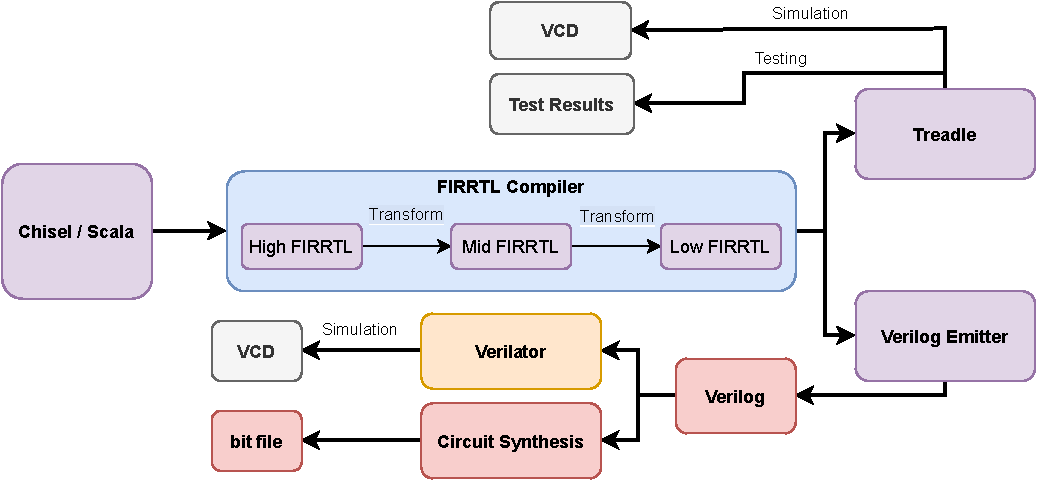
\includegraphics[width=0.8\textwidth]{Chisel_FIRRTL_VERILOG.pdf}
    \caption{Overview of the Chisel pipeline. Chisel code is first given to the FIRRTL compiler, where it is transformed by a series of "lowering passes". It is then output by the compiler in a low-level form, where only hardware primitives are used without loops. It is then used to either emit Verilog or simulate using an execution engine like Treadle.}
\label{fig:chisel}
\end{figure*}

\subsection{FIRRTL}
In a Chisel design, the source code is first compiled into an intermediate representation, named Flexible Intermediate Representation for RTL (FIRRTL), that is used as a sort of ``optimization layer" before being converted into the final Verilog form. During this optimization process the original Chisel description goes through three different intermediate representation layers:
\begin{itemize}
\item High-FIRRTL, which is a form that maps perfectly back to Chisel, but with the FIRRTL structure.
\item Mid-FIRRTL, which is a form where abstract constructs are simplified, i.e., loops are unrolled and arrays are flattened.
\item Low-FIRRTL, which maps to RTL code with high-level conditional statements turned into multiplexers.
\end{itemize}
Throughout this optimisation process, custom FIRRTL compiler passes, known as \textit{Transforms}, can be used to modify the design. This is often done when trying to apply simplifications to the design to make the generated hardware more optimal~\cite{firrtl}.  

Figure~\ref{fig:chisel} shows an overview of the Chisel compilation pipeline and the different stages the code goes through before being converted into a usable format.

\subsection{Code Coverage}
In software development, code coverage is used as a metric to measure the completeness of a testing suite. In recent years, these techniques, originally used for software, have been brought into the hardware verification universe. The coverage metric can be defined in multiple ways, but in this paper we will mostly focus on two key aspects of it: statement coverage and functional coverage. 
%Nonetheless, we briefly mention closely related and more thorough coverage metrics here.

\paragraph{Statement Coverage.} When wanting to retrieve coverage information about a specific program or design, statement coverage will give us a quantitative measure of our testing progress. It measures which percentage of statements in our code have been tested. This metric can be very useful in the software world, when it comes to completeness of a testing suite, however it is only a partial solution in the hardware world, since it only tells us which lines were tested and not how well they were tested.

Related metrics are line and block coverage. Line coverage measures execution of specific code lines. For languages that are less expressive than Scala (such as C), line and statement coverage are equivalent metrics. Block coverage simply reduces the granularity focusing on sections of code at once. Depending on the language, blocks may be explicit or implicit; as an example, consider the code snippets below. The left snippet is written in Verilog and presents an explicit block surrounded by an \texttt{if}-statement whose check may never be true, while the right snippet is written in VHDL and presents an implicit block starting with the \texttt{wait}-statement which may never be passed \cite{hdlverify}.

\noindent\begin{minipage}{.45\textwidth}
\begin{lstlisting}[language=verilog]{verilogBlock}
if (dtack == 1'b1) begin: acked
    as <= 1'b0;
    data <= 16'hZZZZ;
    bus_rq <= 1'b0;
    state <= IDLE;
end
\end{lstlisting}
\end{minipage}\hfill
\begin{minipage}{.45\textwidth}
\begin{lstlisting}[language=vhdl, firstnumber=1]{vhdlBlock}
address <= h"FFED";
ale     <= '1';
rw      <= '1';
wait until dtack = '1';
read_data := data;
ale     <= '0';
\end{lstlisting}
\end{minipage}

More elaborate metrics include path and expression coverage. Figure~\ref{fig:expr} shows examples of both. Path coverage focuses on whether all possible paths through a piece of code have been executed. 
%This is most easily exemplified with an \texttt{if}-statement.
Expression coverage takes this one step further checking whether all possible combinations of true checks are executed. The left code snippet in Figure~\ref{fig:expr} shows an example of path coverage, while the right code snippet shows expression coverage. One must note that the finer the granularity, the greater the computational requirements. For simple designs, statement coverage is generally sufficient \cite{hdlverify}.

\begin{figure}
    \centering
    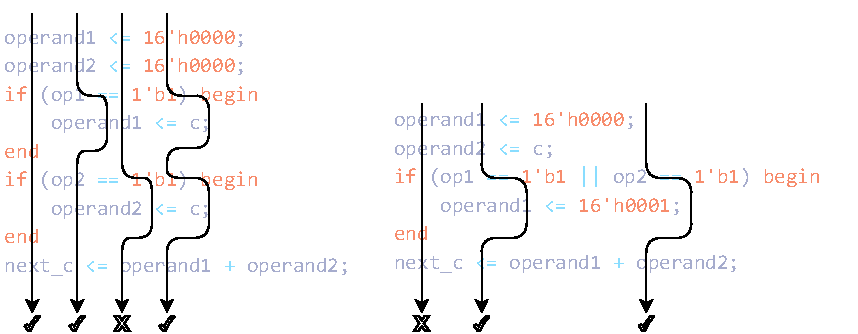
\includegraphics[width=0.5\textwidth]{Coverage_example.pdf}
    \caption{Example of path and expression coverage}
\label{fig:expr}
\end{figure}

\paragraph{Functional Coverage.} If we are looking to measure the completeness of a test suite, we need to ask the following question: \textit{``Are we even testing the right thing?"}. In the hardware world, engineers usually implement designs based on pre-determined specifications, so when testing, we should also have a metric for how well we are implementing the specification. Functional coverage covers that testing. The idea is to first define what is called a \textit{Verification Plan}~\cite{spear2008systemverilog}, which is supposed to represent the specification we are trying to implement. Once that is done, we can then sample the different points defined in the specification during the testing process, to obtain results in the form of: \textit{``test suite T covered a total of x\% of the values specified by point P in specification A"}. This was first implemented in SystemVerilog, in which a verification plan was defined using the following constructs:  
\begin{itemize}
\item \texttt{Bin}: Defines a range of values that should be tested for (i.e., what values can we expect to get from a given port). Whenever the sampled value is within the range defined by a bin, the counter associated with the bin is incremented.
\item \texttt{CoverPoint}: Defines a port that needs to be sampled in the coverage report. These are defined using a set of bins.
\item \texttt{CoverGroup}: Defines a set of \texttt{CoverPoint}s that need to be sampled at the same time.
\end{itemize}
Our solution mimics this verification plan syntax to simplified transition of verification engineers from SystemVerilog to Chisel.

\subsection{What to Aim For}

The greatest pitfall is the idea of needing to hit 100\,\% coverage, regardless of the coverage type considered. Indeed, in the majority of cases, reaching 100\,\% is either unreasonable due to the computational requirements (exhaustively testing a 2-input $n$-bit adder requires $2^{n+1}$ different input patterns!) or impossible due to statements not meant to be executed (e.g., assertions or default cases in fully-specified switch statements). Hence, one should generally aim not for a specific percentage but rather fully exercising the most important code blocks of one's design.

Additionally, we should keep in mind that coverage metrics solely indicate the thoroughness of the verification suite. They provide no indication of the correctness or completeness of the suite. That is, they give no information on whether the design under test (DUT) is correctly functioning, merely how much it was exercised~\cite{hdlverify}.

\subsection{Coverage in Chisel} Up until recently, the main Chisel developers have mostly focused their energy on getting Chisel up to the standards imposed by mainstream HDLs like VHDL or Verilog. This means that verification features are mostly lacking from the Chisel package. Some testing frameworks like \textit{ChiselTest}~\cite{chisel:tester2} have come to be, but they still lack coverage capabilities. All of this amounts to the realisation that if one wants to gather code coverage of a current Chisel design, we need to rely on basic Scala software code coverage tools (which we explore in more detail in a later section). Therefore, we introduce code coverage solutions that are specifically tailored for Chisel.

\subsection{Coverage in SystemVerilog}
SystemVerilog is the de-facto standard for verification. It supports functional coverage and assertions, and is widely used in the scope of the Universal Verification Methodology (UVM). 

As was previously discussed, when performing functional verficiation in SystemVerilog, a \texttt{CoverGroup} is used to group related signals that should be sampled at the same time, a C\texttt{overPoint} specifies the signals which are of interest, and the bins specify what ranges of values are of interest.

Consider below an example where an ALU is tested to ensure that all operations have been performed with all edge-case values (0, 1, -1 etc).
When declared without any explicitly instantiated bins, the coverpoint \texttt{OPS}, covering the signal \texttt{op}, will auto-generate one bin for each possible value that the signal may take on. The coverpoint \texttt{DIN} explicitly declares bins for the values of interest, and declares a bin \texttt{others} to collect all remaining test input which are not an edge case.

\begin{lstlisting}[language=verilog]
covergroup all_ops_edge_cases;
  OPS: coverpoint op;

  DIN: coverpoint din {
    bins min_value = {32'h80000000};
    bins neg1 = {'1};
    bins zero = {0};
    bins one =  {1};
    bins max_value = {32'h7fffffff};
    bins others = default; // All the rest
    }
endgroup: all_ops_edge_cases
\end{lstlisting}

SystemVerilog also supports cross coverage, a special kind of coverpoint which is only incremented whenever two or more coverpoints have specific values. The cross between two coverpoints automatically generates bins for all possible bin combinations. If a coverpoint with 3 bins is crossed with a coverpoint with 8 bins, the resulting cross coverage point would have 24 bins.

%Below is shown an example where we ensure that all of the ALU operands function correctly in the clock cycle where the reset signal has toggled from 1 to 0.

%\begin{lstlisting}[language=verilog]
%covergroup post_rst;
%  UPDOWN: coverpoint reset {
%    bins updown = (1 => 0);
%  }
%  
%  OPS: coverpoint op;
%  cross UPDOWN, OPS;
%endgroup: post_rst
%\end{lstlisting}

%In this example, the bin \texttt{updown} is incremented every time the reset signal toggles from 1 to 0. The current operation is sampled on every clock cycle.  By verifying that all bins have at least one hit, it can be concluded that all operations have been attempted at least once directly following a reset. 

Coverage is sampled whenever the \texttt{sample} method is called on a covergroup. This may be on every clock cycle, or dependent on a chosen event such as the current state of the DUT. Below we show an example function which is called once per clock cycle, taking a container object which contains the values currently on the DUT bus as a parameter. These are copied into variables local to the coverage object, and the covergroups are sampled. Notice that these local variables are the variables used when defining the covergroups.

\begin{lstlisting}[language=verilog]
function void coverage_sample(container c);
	op = c.op;
	din = c.din;
	reset = c.reset;
	
	all_ops_edge_cases.sample();
	post_rst.sample();
endfunction;
\end{lstlisting}

Once the test has been run, a coverage report may be generated by the simulator. If a covergroup has 100\% coverage, all relevant values have been covered. If not, this may indicate that the design is missing some functionality.

%Now that the sufficient background was presented, we can move on to presenting the different methods that allow for statement coverage gathering on a Chisel design at three different abstraction levels.

%\martin{I would change the order from high level to low level:
%1. Chisel source, 2. FIRRTL, 3. Verilog (verilator).
%BTW: we could in principle use vcs to do the Verilog level.} Fixed.

\section{Applying Existing Tools}

\subsection{Statement Coverage at the Scala Level}
\andrew{Maybe we should consider shortening this section and moving it into the background section, since it isn't really one of our contributions and is more an exploration of current methods.}
We will start with measuring coverage at a high level (i.e., coverage of the Scala/Chisel code itself), which gives code coverage to test the hardware generators. Scala and ScalaTest have some coverage functionalities for software testing built-in, specifically, we have looked at the Scoverage plugin which is available with ScalaC through SBT and Maven \cite{scoverage}. Scoverage supports statement and branch coverage rather than simple line coverage. We note that according to the Chisel3 GitHub wiki-page, Scoverage should work with Chisel \cite{chisel:scoverage}.

%\martin{This actually does coverage of the Chisel hardware generation, not the Chisel hardware itself. It tests the generator, which is important as well.} Fixed.

\subsubsection{Using the Scoverage Plugin}
To enable coverage, the Scoverage plugin must be added to the Scala project, including optional arguments.
%'s \textit{plugins.sbt} file, and a number of optional arguments may be included in the project's \textit{build.sbt} file -- the arguments specify whether coverage is enabled, a targeted coverage percentage, etc.
An example configuration is provided below:
\begin{verbatim}
coverageEnabled := true
coverageMinimum := 70
coverageFailOnMinimum := false
coverageHighlighting := true
\end{verbatim}
% Running a test is still just a matter of running e.g. \texttt{sbt test}, while generating a coverage report requires running \texttt{sbt coverageReport} afterwards, as Scoverage otherwise simply generates coverage databases.
Running the test and coverage report will create a set of HTML files. The page may optionally include the original source files with statements that were executed during the test marked in green. The global coverage results are also printed to \texttt{stdout}.
%in the terminal:
%\begin{verbatim}
%[info] Statement coverage.: 100.00%
%[info] Branch coverage....: 100.00%
%\end{verbatim}

\subsubsection{Scoverage Limitations}
While the previous section seems promising, experimenting with Scoverage in combination with Chisel revealed some limitations. In particular, some of the basic constructs introduced by Chisel, e.g. \texttt{switch} statements, are simply not considered by the Coverage tool and thus, incomplete results are reported. In practice, this makes Scoverage insufficient for hardware verification. However, it must be noted that Scoverage provides coverage results for the hardware generators written in Chisel, which can also be important to consider, both for verification and potentially for optimization purposes by pointing a designer's attention toward unused generator code.

\subsection{Statement Coverage at the Verilog Level}

\martin{We will drop this section and move it to one paragraph in related work,
mention the HTML generation, and reference Enricos' thesis}


\andrew{We can also move this part up, directly separating our direct contributions and our exploration of existing methods, as one of the reviewers advised.}
An other solution to obtaining statement coverage, is to rely on the generated Verilog. Since Chisel as a language is not directly supported by any synthesis tools, it relies on transforming the intermediate representation of the FIRRTL stage into Verilog. The Verilog code generated can then be simulated by any Verilog simulator or directly synthesized by any vendor-specific development tool. As part of the Chisel development tools, \texttt{ChiselTest} is a library based on \texttt{ScalaTest}~\cite{ScalaTest}, which allows simulating a Chisel design transformed to Verilog using the Verilator~\cite{verilator} back-end.

Verilator is an open-source simulator guided by the Chips Alliance and Linux Foundation project. Verilator is one of the fastest Verilog simulators available today, outperforming commercial simulators. It is supported and used by numerous companies. It translates Verilog code to C++/SystemC code for the simulation.

%Since version 2.1, Verilator started introducing coverage support.
The current version of Verilator (4.108) supports three types of coverage: line coverage, toggle coverage, and SystemVerilog assertions property coverage. The recording of the coverage can be enabled during the translation from Verilog to C++ code.
%by invoking the Verilator binary with the \textit{--coverage-line}, \textit{--coverage-toggle}, \textit{--coverage-user} parameters, respectively. A fourth parameter called \textit{--coverage} is available to the users, and it enables all three types of coverage simultaneously.

The \textit{coverage-line} parameter is used to specify coverage analysis for each code flow change point in the Verilog source code~\cite{verilatormanual}. For each of these decision points, a counter is kept and incremented every time the specific path is taken during the simulation. The \textit{coverage-toggle} parameter enables the analysis of every signal in a module. With this parameter enabled, every signal that is not local to the module has a counter that increments every time the signal changes states. Lastly, the \textit{coverage-user} parameter enables user-defined functional coverage in the form of SystemVerilog assertions. This type of coverage is not considered in this report since it requires manual intervention from the user or implementing a custom transformation for inserting SystemVerilog assertion in the generated Verilog code through FIRRTL annotation.

When the simulation is run with coverage enabled, Verilator generates a coverage report in a SystemPerl~\cite{SystemPerl} coverage report file.
%for each different test at the end of the simulation. The output of multiple tests can then be combined by using the \textit{verilator\_coverage} utility provided with Verilator. The merged report file can then be transformed into an info file and processed by any coverage tools or extensions.

One of the most used front ends for code coverage is LCOV~\cite{Lcov}. LCOV is a graphical front end developed as part of the Linux test project, and it can read coverage results and display them in the form of an HTML page through its companion utility genhtml. As part of Google Summer Of Code 2014, genhtml was ported to Java by Rick Brown under the name jgenhtml~\cite{jgenhtml}.

By combining genhtml, Verilator, and \texttt{ChiselTest}, it is possible to automatically generate a coverage report for each test suite specified inside \texttt{ChiselTest}. We extended the \texttt{ChiselTeste} library with a custom ScalaTest reporter generator that automatically detects the coverage files generated by Verilator, merges them, and creates an HTML page reporting the source code of the module tested and displaying which lines were covered during the run of the test suite.

When a user creates a test suite that mixes in the Scala trait \texttt{CoverageTrait} an output similar to the one below will be printed at the end of the test:
\begin{lstlisting}[language=bash]
Reading data file: output.info
Found common filename prefix /Users/enrico/Documents/Git/transfer/output/uvm/
Generating output at [...]/transfer/output/uvm/chisel.AluAccuTester
Writing report for AluAccuChisel.v
Writing directory view page.
Overall coverage rate:
	lines......: 100.0% (13 of 13 lines)
	functions: no data found
	branches: no data found
Line coverage 100.0%, Coverage saved in file:///
[...]/output/uvm/chisel.AluAccuTester/VerilatorCoverage.html
[info] ScalaTest
[info] Run completed in 6 seconds, 258 milliseconds.
[info] Total number of tests run: 7
[info] Suites: completed 5, aborted 0
[info] Tests: succeeded 7, failed 0, canceled 0, ignored 0, pending 0
[info] All tests passed.
[info] Passed: Total 7, Failed 0, Errors 0, Passed 7
[success] Total time: 12 s, completed Dec 10, 2020 9:24:46 PM
\end{lstlisting}

The HTML output is shown in Figure~\ref{fig:customhtmlreport}.

\begin{figure*}
\centering
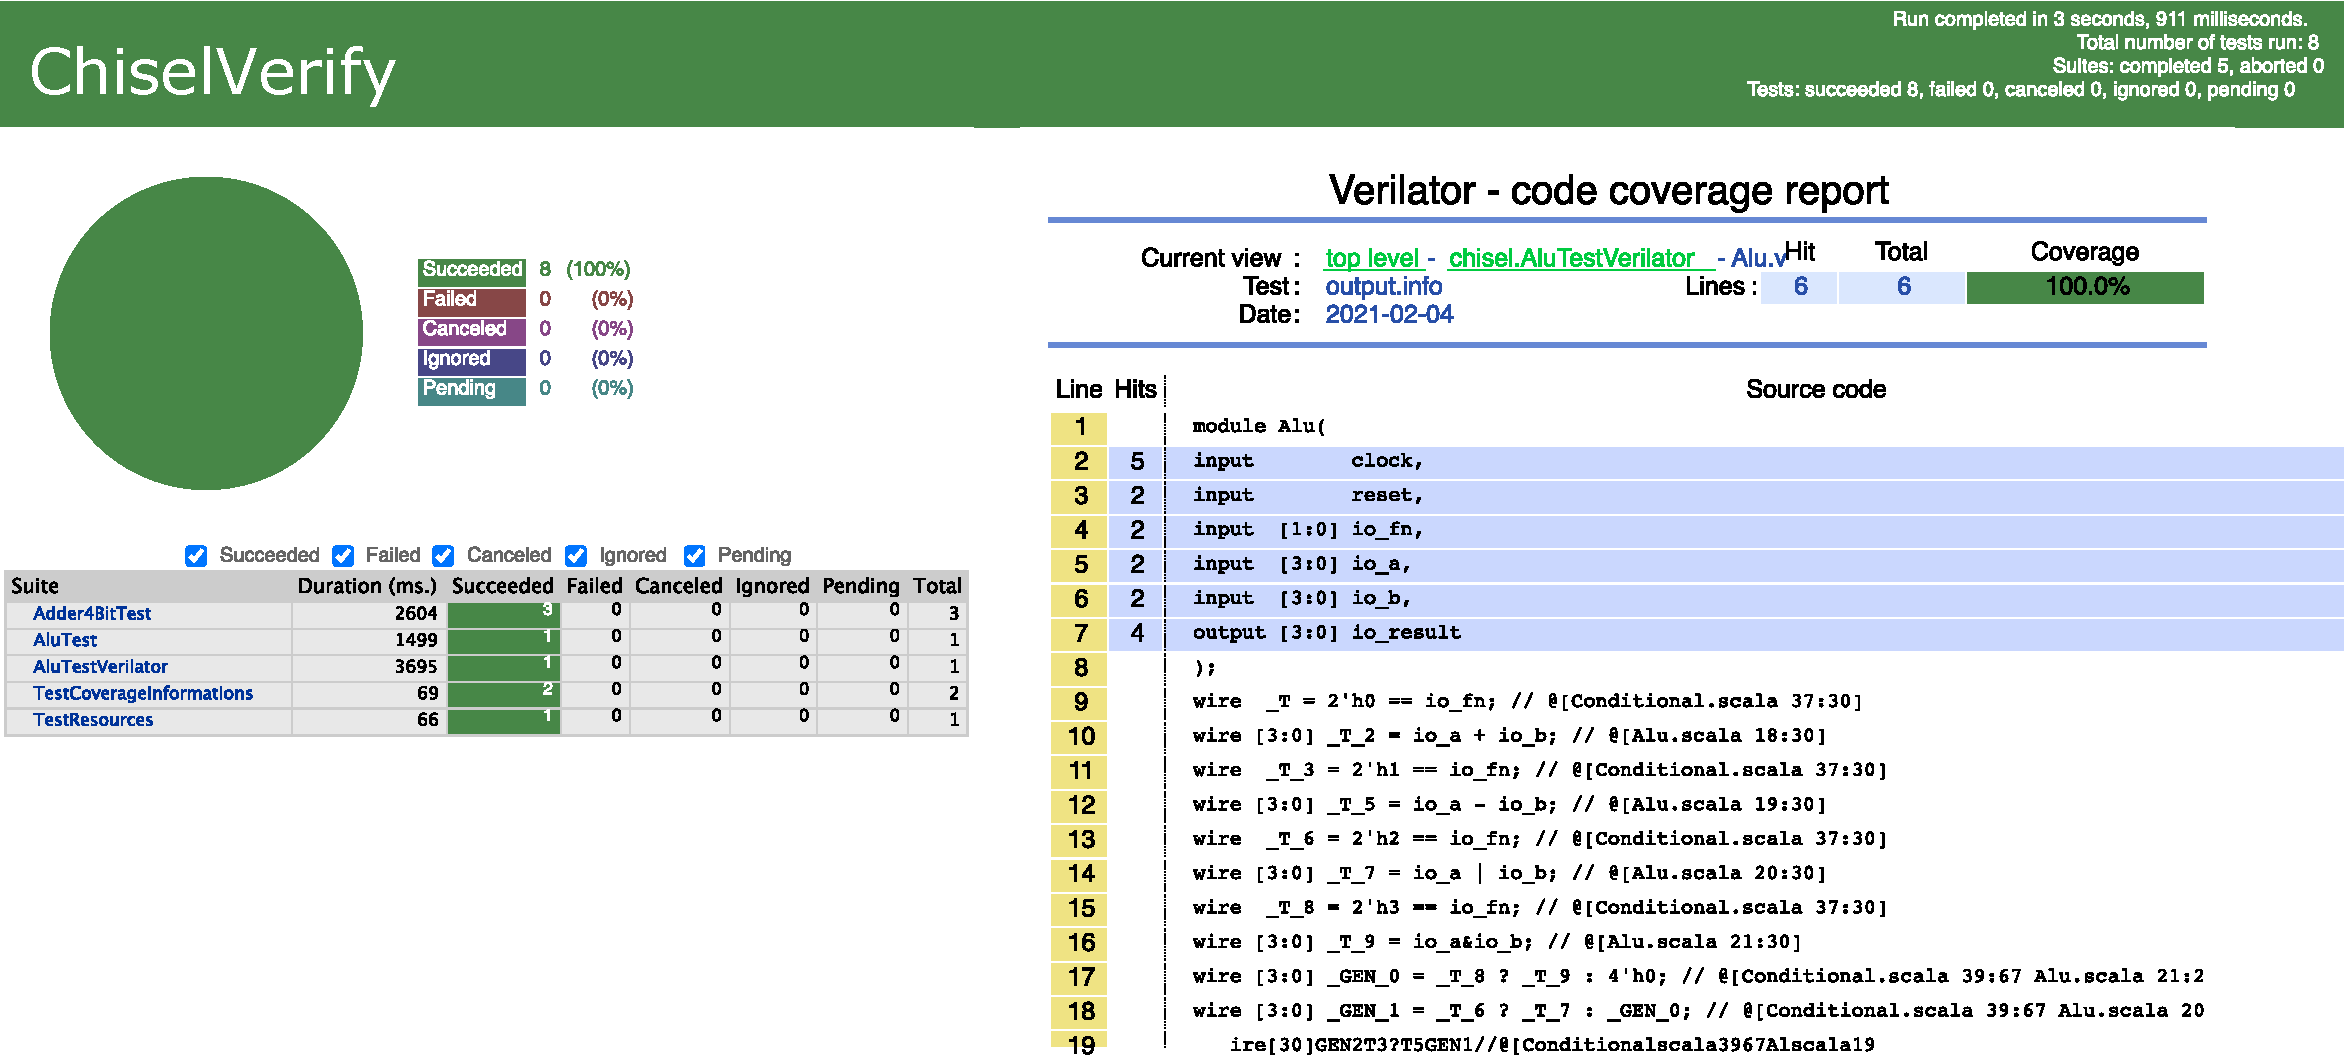
\includegraphics[width=0.8\textwidth]{ChiselverifyHtml.pdf}
\caption{Custom HTML ChiselTest report with Verilator coverage}
\label{fig:customhtmlreport}
\end{figure*}


\section{Statement Coverage at the FIRRTL Level}  
%Let us now move down an abstraction level and discuss how we've gone about implementing statement coverage at the FIRRTL level. First of all, we must briefly discuss the utility of having coverage at an intermediate representation level.
FIRRTL is a direct translation of the input Chisel source, meaning that it can be mapped intuitively back to the designer's code. An argument for the usefulness of coverage information at such an abstraction level is the fact that in FIRRTL, all hardware generators are expanded, meaning that what we see this information on the generated hardware rather than the hardware generating code. 

We developed new methods allowing for coverage measurements in Treadle, a common FIRRTL execution engine used to simulate designs implemented in Chisel. This engine runs on the FIRRTL intermediate representation code generated by a given Chisel implementation and allows to run user-defined tests on the design, using frameworks like \texttt{iotesters} or the more recent \texttt{ChiselTest}. One way to obtain FIRRTL-level statement coverage would be to run our tests through an extended version of Treadle (available through a SNAPSHOT at the time of writing) capable of keeping track of the necessary information.

The solution that was used to implement statement coverage is based on a method presented by Baxter~\cite{branch-cov-made-easy:2002}. The idea is to add additional outputs for each multiplexer in the design. These new ports, which we will call \textit{Coverage Validators}, are set depending on the paths taken by each multiplexer. That information is then gathered at the end of each test and maintained throughout a test suite. Once the testing process is finished, we use the output values gathered from the \textit{Coverage Validators} to check whether or not a certain multiplexer path was taken during the test, resulting in a branch coverage percentage. This percentage can then be mapped to a statement coverage percentage.

We developed this method inside of Treadle by creating a custom pass of the FIRRTL compiler, in Scala, that traverses the source's abstract syntax tree and adds the additional outputs and coverage expressions into the data structure. Once that is done, the \texttt{TreadleTester} samples those additional outputs every time the \texttt{expect} method is called and keeps track of their values throughout a test suite. Finally, it generates a Scala \texttt{case class} containing the following coverage information:
\begin{itemize}
\item The multiplexer path coverage percentage.
\item The coverage Validator lines that were covered by a test.
\item The modified LoFIRRTL source code in the form of a \texttt{List[String]}.
\end{itemize}
The \texttt{CoverageReport} case class can then be serialized, giving the following example report:
\begin{verbatim}
COVERAGE: 50.0% of multiplexer paths tested
COVERAGE REPORT:

+ circuit Test_1 :
+   module Test_1 :
+     input io_a : UInt<1>
+     input io_b_0 : UInt<2>
+     input io_b_1 : UInt<2>
+     input clock : Clock
+     output io_cov_valid_0 : UInt<1>
+     output io_cov_valid_1 : UInt<1>
+     output out : UInt<2>
+   
+     io_cov_valid_0 <= io_a
-     io_cov_valid_1 <= not(io_a)
+     out <= mux(io_a, io_b_0, io_b_1)
\end{verbatim}
The example above is taken from a simple test, where we are only testing the path where \texttt{in\_a} is 1. This means that, since we only have a single multiplexer, only half of our branches have been tested and we would thus want to add a test for the case where \texttt{in\_a} is 0. The report can thus be interpreted as follows:  
\begin{itemize}
\item ``\texttt{+}" before a line, means that it was executed in at least one of the tests in the test suite. All port declarations are considered explored by default.
\item ``\texttt{-}" before a line, means that it wasn't executed in any of the tests in the test suite. This can only appear next to a line containing a coverage-validator, since it represents a non-explored multiplexer path.
\end{itemize}

With our modification Treadle thus allows us to obtain coverage at the FIRRTL level. An interesting result can be obtained by mapping the FIRRTL statement coverage to the original Chisel source. This is possible by accessing the original source code through \textit{Source locators} which map some of the FIRRTL lines back to Chisel.
%Another way to obtain coverage information would be to use the generated Verilog description and we will discuss that in detail in the following section.

\martin{Maybe we should lookup what Kevin is doing. Kind of picked up our work.}

\section{Functional Coverage in Chisel}

\martin{This is our main contribution, so expand on this.}

Functional coverage is one of the principal tools used during the verification process. It allows one to measure \textit{``which part of the specification has been implemented correctly"}. A discussion on hardware verification would thus not be complete without constructs allowing one to define a verification plan and retrieve a functional coverage report. The main language used for functional coverage is usually SystemVerilog, which is why our solution is based on the same syntax. 

Functional coverage is based on three base elements: \texttt{Bins}, \texttt{CoverPoints} and \texttt{CoverGroups}. Using these, one can define what's known as a verification plan, which tells the coverage reporter what ports need to be sampled and taken into account in the coverage report.
In order to implement said elements in Scala, we needed to be able to do the following:
\begin{itemize}
\item Define a verification plan (using constructs similar to \texttt{coverpoint} and \texttt{bins}).
\item Sample DUT ports (for example by hooking into the \textit{ChiselTest} framework).
\item Keep track of the number of hits that a bin has obtained (using a sort of a database).
\item Compile all of the results into a comprehensible coverage report.
\end{itemize}

We implemented this on top of the existing \texttt{ChiselTest}~\cite{chisel:tester2} framework, using a structure similar to the one used in SystemVerilog~\cite{spear2008systemverilog}. We start with a top-level construct, called \texttt{CoverageReporter}, which allows one to define a verification plan using the \texttt{register} method, which itself stores the \texttt{coverpoint} to \texttt{bin} mappings inside of a \texttt{CoverageDB}. Once the verification plan is defined, we can sample the DUT ports using the \texttt{sample} method, which hooks into \texttt{ChiselTest} in order to use its peeking capabilities. At the end of the test suite, a functional coverage report can be generated using the \texttt{printReport} method, which shows us how many of the possible values, defined by our bin ranges, were obtained during the simulation.

\begin{lstlisting}[language=scala]
val cr = new CoverageReporter
cr.register(
    // Declare CoverPoints
    // CoverPoint 1
    CoverPoint("accu", dut.io.accu)(
        Bins("lo10", 0 to 10),
        Bins("First100", 0 to 100)
     ),
    // CoverPoint 2
    CoverPoint("test", dut.io.test)(
        Bins("testLo10", 0 to 10)
     ),
    // Declare cross points
    Cross("accuAndTest", dut.io.accu, dut.io.test)(
        CrossBin("both1", 1 to 1, 1 to 1)
     )
)
\end{lstlisting}
The above code snippet is an example of how to define a verification plan using our Scala solution. Note that the semantics follow that of \texttt{SystemVerilog}:
\begin{itemize}
    \item \texttt{CoverGroup} is defined as a list of \texttt{CoverPoint}s using the \texttt{cr.register} method.
    \item \texttt{CoverPoint} is defined as a list of \texttt{Bins} tied to a DUT port and a name. If no \texttt{Bins} are given, then a \texttt{DefaultBin} is used, ranging over all possible values for the given port.
    \item \texttt{Bins} instance is defined by a name and a value range.
    \item \texttt{CrossPoint} is defined using the names of two previously defined \texttt{CoverPoints} and a list of \texttt{CrossBins}.
    \item \texttt{CrossBins} instance is defined using two ranges given in the same order as their associated \texttt{CoverPoint}.
\end{itemize}
The concepts are directly taken from \texttt{SystemVerilog}, so it should be accessible to anyone coming from that environment. 

\subsection{Generating the Coverage Report}
After defining a verification plan, we need to decide when we want to sample our cover points. This means that at some point in our test, we have to tell our \texttt{CoverageReporter} to sample the values of all of the points defined in our verification plan. This can be done, in our example, simply by calling \texttt{cr.sample()} when we are ready to sample our points. Finally once our tests are done, we can ask for a coverage report by calling \texttt{cr.printReport()} which results in the following coverage report: 
\begin{verbatim}
============== COVERAGE REPORT ==============
================ GROUP ID: 1 ================
COVER_POINT PORT NAME: accu
BIN lo10 COVERING Range 0 to 10 
HAS 8 HIT(S) = 80%
BIN First100 COVERING Range 0 to 100 
HAS 9 HIT(S) = 9%
============================================
COVER_POINT PORT NAME: test
BIN testLo10 COVERING Range 0 to 10 
HAS 8 HIT(S) = 80%
============================================
CROSS_POINT accuAndTest FOR POINTS accu AND test
BIN both1 COVERING Range 1 to 1 CROSS Range 1 to 1 
HAS 1 HIT(S) = 100%
============================================
\end{verbatim}
Another option would be, for example if we want to do automated constraint modifications depending on the current coverage, to generate the coverage as a Scala \texttt{case class} and then to use its \texttt{binNcases} method to get numerical and reusable coverage results.  
  
\subsection{Timed Coverage}
\andrew{This can be much more developed}
One final element that our framework offers is the possibility to gather delayed coverage relationships between two coverage points. The idea is similar to how a \texttt{Cross} works, but this time rather than sampling both points in the same clock cycle, we look at the relation between one point at the starting clock cycle and another point sampled a given number of clock cycles later. This number of clock cycles is called the \texttt{delay} and there are currently three different ways to specify it:  
\begin{itemize}
 \item \texttt{Exactly} delay, means that a hit will only be considered if the second point is sampled in its range a given number of cycles after the first point was.
 \item \texttt{Eventually} delay, means that a hit will be considered if the second point is sampled in its range at any point within the following given number of cycles after the first point was.  
 \item \texttt{Always} delay, means that a hit will be considered if the second point is sampled in its range during every cycle for a given number of cycles after the first point was sampled.
\end{itemize}  

\andrew{We should probably also have a section that talks about the purely conditional coverage.}

%This thus concludes our discussion on Functional Coverage. We will now move on to presenting an industry provided use-case and show how our coverage solutions can be used to improve the testing efficiency of Chisel designs.

\section{Evaluation}

\martin{Could be more}

As a way of evaluating our coverage solution in Scala, a use-case provided by Microchip was developed and verified using the functional coverage constructs presented in the previous section. It also gave the opportunity to assess how well a complete design process conducted only in Scala/Chisel works with the added features. The use-case is a heap-based priority queue which is meant to be used for scheduling purposes in real-time systems. Values referring to a specific clock cycle number in a specific super cycle can be inserted as well as removed. The priority queue sorts all enqueued values such that the value referring to the next clock cycle number that will be encountered is presented to the host system. 

The \texttt{ChiselTest} framework was used for testing (using a peek/poke/expect interface) and our functional coverage solution was used to verify the use-case. Defining the verification plan in Scala was done using the following structure:  
\begin{lstlisting}[language=scala]
val cr = new CoverageReporter(c)
cr.register(
    CoverPoint("operation", c.io.cmd.op)(
        Bins("insertion", 0 to 0),
        Bins("removal", 1 to 1)
    )//More CoverPoints
)
\end{lstlisting}
In total we defined 5 \texttt{CoverPoints} each having up to 3 bins and 2 \texttt{CrossPoints} each having up to 5 cross bins. This was done in roughly 20 lines of Scala, meaning that once the verification plan was defined, we can simply sample it directly inside of our \texttt{ChiselTest} code without ever having to leave the Chisel/Scala world.

Another solution would have been to gather the functional coverage in SystemVerilog rather than in Scala. This however means that Chisel testing frameworks, such as \texttt{ChiselTest} could not have been used, since all of the testing would have to be done in SystemVerilog. For the sake of the argument, let's suppose that only the functional coverage gathering needed to be done in SystemVerilog, then the following would have had to be done in order to obtain the same result as our Scala-based solution:  
\begin{itemize}
    \item Create a UVM-subscriber based coverage class.
    \item Instantiate the current DUT (\texttt{priorityQueue pQ  = new;})
    \item Declare the verification plan: 
    \begin{lstlisting}[language=verilog]
covergroup unnamed;
	OPERATION: coverpoint pQ.cmd.op {
		bins insertion = {0};
		bins removal = {1};
		//More bins
	}
	//More coverpoints
endgroup: unnamed;
    \end{lstlisting}
    \item Define \texttt{build\_phase} and \texttt{write} functions.
    \item Define the coverage class constructor.
\end{itemize}  
All of this sums up to roughly 100 lines of code for the same result. So not only does our solution allow us to perform the entirety of our design and verification within the same ecosystem (moving to SystemVerilog would first require to generate Verilog from the Chisel design and then to simulate it using a SystemVerilog capable simulator like Verilator), but it also reduces the 5 step functional coverage process to a single step (defining the verification plan). It thus requires much less boilerplate code and reduces the total source code by a factor of 5.  

The Scala functional coverage solution presents itself as a natural addition to the \texttt{ChiselTest} framework. One of the main advantages here is that the same language can be used for design and verification, thus increasing the time effectiveness and removing a possible source of errors. Overall, the use-case makes a strong point for hardware development in Scala/Chisel and all the possibilities that come with it. The coverage features, for both functional and statement coverage, help pave the way to a fully capable verification suite accompanying the Chisel language.



\section{Conclusion}
We propose multiple solutions for the gathering of coverage data in high-level Chisel designs. Previously, one needed to rely on other languages such as SystemVerilog in order to obtain coverage information during the verification of a Chisel design. This meant that testing either needed to be done in another language or we needed to turn to multi-language testing which was very often cumbersome and time-consuming. With our solutions we are bringing the world one step closer to making Chisel a fully capable design and verification language.
We presented several methods of collecting coverage measurements staying within Scala/Chisel.
%We now no longer need to rely on other languages in order to gather statement and functional coverage of our Chisel designs. An interesting discussion to be had is around the abstraction-level that should be used to gather coverage. One could justify that high-level coverage information lacks usefulness when using hardware generators since we would rather have information on the execution of the generated hardware rather than the generator itself, but of course this discussion is left up for the reader to have. 

\section*{Acknowledgements}
We would like to thank the researchers at Berkeley who are constantly working on making Chisel a more ubiquitous hardware construction language and for the feedback related to the work done on adding coverage to Treadle.

\subsection*{Source Access}

\todo{Add source pointers in final version. Not possible now due to double-blind review.}

\bibliographystyle{IEEEtran}
\bibliography{coverage,../msbib,../funding/ftp-chisel/testing,../chisel-uvm}
\end{document}
